% !TEX TS-program = pdflatex
% !TEX encoding = UTF-8 Unicode

% This file is a template using the "beamer" package to create slides for a talk or presentation
% - Giving a talk on some subject.
% - The talk is between 15min and 45min long.
% - Style is ornate.

% MODIFIED by Jonathan Kew, 2008-07-06
% The header comments and encoding in this file were modified for inclusion with TeXworks.
% The content is otherwise unchanged from the original distributed with the beamer package.

\documentclass{beamer}


% Copyright 2004 by Till Tantau <tantau@users.sourceforge.net>.
%
% In principle, this file can be redistributed and/or modified under
% the terms of the GNU Public License, version 2.
%
% However, this file is supposed to be a template to be modified
% for your own needs. For this reason, if you use this file as a
% template and not specifically distribute it as part of a another
% package/program, I grant the extra permission to freely copy and
% modify this file as you see fit and even to delete this copyright
% notice.


\mode<presentation>
{
  \usetheme{Warsaw}
  % or ...

  \setbeamercovered{transparent}
  % or whatever (possibly just delete it)
}

\usepackage[vietnam]{babel}
% or whatever

\usepackage[utf8]{inputenc}
% or whatever

\usepackage{times}
\usepackage[T1]{fontenc}
\usepackage{color}
\usepackage{graphicx}
\usepackage[font=Times,timeinterval=1, timedeath=0]{tdclock}
%\usepackage{multimedia}
% Định nghĩa các tiêu đề
\renewcommand{\chaptername}{Chương}
\renewcommand{\appendixname}{PHỤ LỤC}
\newcommand{\hty}{\rightharpoonup}
\newcommand{\rong}{\emptyset}
\newtheorem{tm}{ }
\newtheorem{dn}{\large Định nghĩa}[section]
\newtheorem{dly}{\large Định lý}[section]
\newtheorem{chy}{\large Chú ý}[section]
\newtheorem{bd}{\large Bổ đề}[section]
\newtheorem{md}{\large Mệnh đề}[section]
\newtheorem{hq}{\large Hệ quả}[section]
\newtheorem{ly}{\large Lưu ý}[section]
\newtheorem{thm}{Theorem}[section]
\newtheorem{lem}[thm]{Lemma}
\newtheorem{eg}[thm]{Example}
\newtheorem{prop}[thm]{Proposition}
\newtheorem{cor}[thm]{Corollary}
\newtheorem{defn}[thm]{Definition}
\newtheorem{rem}[thm]{Remark}
\newtheorem{ntn}[thm]{Notation}
\newenvironment{prf}{{\noindent \textbf{Proof:}\ }}{\hfill $\Box$\\ \smallskip}
\numberwithin{equation}{section}
\renewcommand{\dateseparator}{--}
%Định nghĩa màu cho chữ viết, các bạn không nên  xóa bỏ phần này

\newcommand{\doo}[1]{\textcolor{red}{#1}}
\newcommand{\xanh}[1]{\textcolor{green}{#1}}
\newcommand{\tim}[1]{\textcolor{violet}{#1}}
\newcommand{\duong}[1]{\textcolor{blue}{#1}}
\newcommand{\bich}[1]{\textcolor{cyan}{#1}}
\newcommand{\hong}[1]{\textcolor{magenta}{#1}}
\newcommand{\vang}[1]{\textcolor{yellow}{#1}}
\newcommand{\trang}[1]{\textcolor{white}{#1}}
\newcommand{\refe}[1]{
\setbeamertemplate{footline}
{%
\leavevmode%
\hbox{%
\begin{beamercolorbox}[wd=1\paperwidth,ht=2.5ex,dp=1.125ex,left]{author
in head/foot}%
\centering
\vang{#1}

\end{beamercolorbox}%
}%

\vskip0pt%

\hbox{%
\begin{beamercolorbox}[wd=.9\paperwidth,ht=2.5ex,dp=1.125ex,left]{title
in head/foot}%
%\usebeamerfont{author in head/foot}
\hspace{.1cm}
\tiny{\trang{Một phương pháp lai trích xuất sự kiện và áp dụng vào hệ thống theo dõi tin tức trực tuyến $\mathcal{N}$\texttt{ewSOMoni} }}%\tddate\ \ \tdtime}}
\end{beamercolorbox}%
%
\begin{beamercolorbox}[wd=.6\paperwidth,ht=2.5ex,dp=1.125ex,left]{title
in head/foot}%
$\;$ $\;$ $\;$ $\;$ \insertframenumber/ \inserttotalframenumber
\end{beamercolorbox}%
}%
\vskip0pt%
}
}

\newcommand{\unrefe}[1]{
\setbeamertemplate{footline}
{%
\leavevmode%
\hbox{%
\begin{beamercolorbox}[wd=.54\paperwidth,ht=2.5ex,dp=1.125ex,left]{author
in head/foot}%
\vang{$\;$ $\;$ $\;$ $\;$ HoàngNM -- MạnhHX -- TâmNV}
\end{beamercolorbox}%

%__THEMVAO
\begin{beamercolorbox}[wd=.46\paperwidth,ht=2.5ex,dp=1.125ex,right]{author
in head/foot}%
\vang{UET, VNU $\;$}

\end{beamercolorbox}%
}%

\vskip0pt%

\hbox{%
\begin{beamercolorbox}[wd=.9\paperwidth,ht=2.5ex,dp=1.125ex,left]{title
in head/foot}%

\hspace{.1cm}
\tiny{\trang{Một phương pháp lai trích xuất sự kiện và áp dụng vào hệ thống theo dõi tin tức trực tuyến $\mathcal{N}$\texttt{ewSOMoni}}}
\end{beamercolorbox}%
%
\begin{beamercolorbox}[wd=.6\paperwidth,ht=2.5ex,dp=1.125ex,left]{title
in head/foot}%
$\;$ $\;$ $\;$ $\;$ \insertframenumber/ \inserttotalframenumber
\end{beamercolorbox}%
}%
\vskip0pt%
}


}

%Định nghĩa màu cho khung và chữ viết, các bạn không nên  xóa bỏ phần này
\setbeamercolor{vangxanh}{fg=blue,bg=yellow!20!white}
\setbeamercolor{vangden}{fg=black,bg=yellow!20!white}
\setbeamercolor{vangdo}{fg=red,bg=yellow!20!white}
\setbeamercolor{camden}{fg=black,bg=orange!20!white}
\setbeamercolor{camxanh}{fg=blue,bg=orange!20!white}
\setbeamercolor{bichdo}{fg=red,bg=cyan!15!white}
\setbeamercolor{bichden}{fg=black,bg=cyan!15!white}
\setbeamercolor{hongxanh}{fg=blue,bg=magenta!15!white}
\setbeamercolor{hongden}{fg=black,bg=magenta!15!white}
\setbeamercolor{lado}{fg=red,bg=lime!40}
\setbeamercolor{laden}{fg=black,bg=lime!40}
\setbeamercolor{laxanh}{fg=blue,bg=lime!40}
\setbeamertemplate{caption}[numbered]

\title[Giám sát luồng thông tin]{Một phương pháp lai trích xuất sự kiện và áp dụng vào hệ thống theo dõi tin tức trực tuyến  $\mathcal{N}$\texttt{ewSOMoni}} % (optional, use only with long paper titles)


\author[HoangNM, QuanNS, HieuNQ] % (optional, use only with lots of authors)
{\textsc{\bich{Cán bộ hướng dẫn}} \\[0.1cm] TS Phan Xuân Hiếu \and ThS. Trần Mai Vũ \\[0.2cm] \textsc{\bich{Sinh viên thực hiện}} \\[0.1cm] Nguyễn Sỹ Quân \and Nguyễn Minh Hoàng \\ Ngô Quang Hiểu}
% - Use the \inst{?} command only if the authors have different
%   affiliation.

\institute[Đại học Công Nghệ] % (optional, but mostly needed)
{
%  \inst{1}%
%  Lớp K53C--CLC\\
%  Đại học Công Nghệ
%  \and
%  \inst{2}%
%  \\
  \tim{Phòng thí nghiệm Công nghệ Tri thức -- Đại học Công Nghệ}
}
% - Use the \inst command only if there are several affiliations.
% - Keep it simple, no one is interested in your street address.

%\date[Short Occasion]{\today}
\date{$\;$}
%\subject{Talks}
% This is only inserted into the PDF information catalog. Can be left
% out.
\setbeamertemplate{footline}
{%
\leavevmode%
\hbox{%
\begin{beamercolorbox}[wd=.54\paperwidth,ht=2.5ex,dp=1.125ex,left]{author
in head/foot}%
\vang{$\;$ $\;$ $\;$ $\;$ HoangNM--QuanNS--HieuNQ}
\end{beamercolorbox}%

%__THEMVAO
\begin{beamercolorbox}[wd=.46\paperwidth,ht=2.5ex,dp=1.125ex,right]{author
in head/foot}%
\vang{UET, VNU $\;$}

\end{beamercolorbox}%
}%

\vskip0pt%

\hbox{%
\begin{beamercolorbox}[wd=.9\paperwidth,ht=2.5ex,dp=1.125ex,left]{title
in head/foot}%
%\usebeamerfont{author in head/foot}
\hspace{.1cm}
\tiny{\trang{Một phương pháp lai trích xuất sự kiện và áp dụng vào hệ thống theo dõi tin tức trực tuyến $\mathcal{N}$\texttt{ewSOMoni} }}
\end{beamercolorbox}%
%
\begin{beamercolorbox}[wd=.6\paperwidth,ht=2.5ex,dp=1.125ex,left]{title
in head/foot}%
$\;$ $\;$ $\;$ $\;$ \insertframenumber/ \inserttotalframenumber
\end{beamercolorbox}%
}%
\vskip0pt%
}


% If you have a file called "university-logo-filename.xxx", where xxx
% is a graphic format that can be processed by latex or pdflatex,
% resp., then you can add a logo as follows:

% \pgfdeclareimage[height=0.5cm]{university-logo}{university-logo-filename}
% \logo{\pgfuseimage{university-logo}}



% Delete this, if you do not want the table of contents to pop up at
% the beginning of each subsection:
\AtBeginSubsection[]
{
  \begin{frame}<beamer>{\trang{\LARGE \bf{Nội dung}}}
    \tableofcontents[currentsection,currentsubsection]
  \end{frame}
}


% If you wish to uncover everything in a step-wise fashion, uncomment
% the following command:

%\beamerdefaultoverlayspecification{<+->}
%LOGO
\pgfdeclaremask{fsu}{uet}
\pgfdeclareimage[mask=fsu,width=1cm]{uet}{uet}

\logo{\vbox{\vskip0.1cm\hbox{\pgfuseimage{uet}}}}

\begin{document}
\DeclareGraphicsExtensions{.jpg,.pdf,.mps,.png,.eps}
%\setbeamertemplate{footline}[frame number]
\begin{frame}
  %\initclock
  \titlepage

\end{frame}


\setbeamertemplate{footline}
{%
\leavevmode%
\hbox{%
\begin{beamercolorbox}[wd=.54\paperwidth,ht=2.5ex,dp=1.125ex,left]{author
in head/foot}%
\vang{$\;$ $\;$ $\;$ $\;$ HoangNM--QuanNS--HieuNQ}
\end{beamercolorbox}%

%__THEMVAO
\begin{beamercolorbox}[wd=.46\paperwidth,ht=2.5ex,dp=1.125ex,right]{author
in head/foot}%
\vang{UET, VNU $\;$}

\end{beamercolorbox}%
}%

\vskip0pt%

\hbox{%
\begin{beamercolorbox}[wd=.9\paperwidth,ht=2.5ex,dp=1.125ex,left]{title
in head/foot}%
%\usebeamerfont{author in head/foot}
\hspace{.1cm}
\tiny{\trang{Một phương pháp lai trích xuất sự kiện và áp dụng vào hệ thống theo dõi tin tức trực tuyến $\mathcal{N}$\texttt{ewSOMoni}}}
\end{beamercolorbox}%
%
\begin{beamercolorbox}[wd=.6\paperwidth,ht=2.5ex,dp=1.125ex,left]{title
in head/foot}%
$\;$ $\;$ $\;$ $\;$ \insertframenumber/ \inserttotalframenumber
\end{beamercolorbox}%
}%
\vskip0pt%
}


%
%\begin{frame}
%  \titlepage
%\end{frame}
\begin{frame}
 \frametitle{\trang{\LARGE \bf  Nội dung}}
 \tableofcontents
 %them vao day
\end{frame}



% Since this a solution template for a generic talk, very little can
% be said about how it should be structured. However, the talk length
% of between 15min and 45min and the theme suggest that you stick to
% the following rules:

% - Exactly two or three sections (other than the summary).
% - At *most* three subsections per section.
% - Talk about 30s to 2min per frame. So there should be between about
%   15 and 30 frames, all told.

%Reference

\begin{frame}{Tài liệu tham khảo}
\bibliographystyle{alpha}
\bibliography{bib/mainbib}
%\addbibresource{bib/mainbib}
\end{frame}


\section{Giới thiệu}
	%\subsection{Động lực nghiên cứu}
    \begin{frame}{Động lực nghiên cứu}
      \begin{itemize}
        \item Thông tin về một sự kiện nổi bật:
          \begin{itemize}
            \item Nhiều
              \item Đa chiều
               \item Tính cập nhật cao
            \end{itemize}
          \medskip
          \pause
        \item Trích xuất sự kiện có vai trò quan trọng:
          \begin{itemize}
            \item Hệ thống theo dõi, giám sát
              \begin{itemize}
                \item BioCaster (\href{http://born.nii.ac.jp/}{http://born.nii.ac.jp/})
                 % \item HealthMap (\href{http://www.healthmap.org/en/}{http://www.healthmap.org/en/})
                    \item EpiSpider (\href{http://www.epispider.org/}{http://www.epispider.org/})
                      \item Metro Monitor (\href{(www.metromonitor.com/}{(www.metromonitor.com/})
                \end{itemize}
              \pause
              \item Hệ thống cảnh báo, bảo mật
                \begin{itemize}
                  \item Frontex (\href{http://www.frontex.europa.eu/}{http://www.frontex.europa.eu/})
                  \end{itemize}
          \end{itemize}
        \end{itemize}
      \end{frame}


    %\subsection{Bài toán đặt ra}
    \begin{frame}{Mô tả bài toán}
      \begin{itemize}
       \item Trích xuất sự kiện theo phương pháp kết hợp luật ngữ nghĩa  và học máy Maximum Entropy
\pause
\item Áp dụng thử nghiệm cho hệ thống theo dõi tin tức
         \begin{itemize}
           \item \textsc{Hình sự}
             \item \textsc{Tai nạn giao thông}
               \item \textsc{Cháy nổ}
          \end{itemize}
        \medskip
        \pause
        \item \textbf{Đầu vào:} một tin tức thu thập trực tuyến
          \pause
        \item \textbf{Đầu ra:}
          \begin{itemize}
            \item Bản tin chứa sự kiện không?
              \pause
              \item Thông tin sự kiện:
                \begin{itemize}
                  \item dạng sự kiện, tên sự kiện
                    \item nhân tố tham gia, thời gian, địa điểm
                 \end{itemize}
          \end{itemize}
      \end{itemize}
    \end{frame}

	%\subsection{Mục tiêu nghiên cứu}
    \begin{frame}{Mục tiêu nghiên cứu}
      \begin{itemize}
        \item Thế nào là sự kiện, trích xuất sự kiện?
          \medskip
          \item Các hướng tiếp cận giải quyết bài toán trích xuất sự kiện?
            \medskip
          \item Làm thế nào để trích xuất sự kiện trên tin tức tiếng Việt?
            \medskip
          \item Một hệ thống theo dõi tin tức có khả thi không?
        \end{itemize}

      \end{frame}


\section{Phương pháp giải quyết}
  \subsection{Các hướng  tiếp cận}
  \begin{frame}{Áp dụng luật}

    \end{frame}

  \begin{frame}{Áp dụng học máy -- thống kê}

    \end{frame}

  \begin{frame}{Kết hợp luật và học máy -- thống kê}

    \end{frame}
  \subsection{Phương pháp đề xuất}




\section{Hệ thống $\mathcal{N}$\texttt{ewSOMoni}}

 \subsection{Mô tả hệ thống}
  \begin{frame}{Mô hình hệ thống}
   % \framezoom<1><2>(2cm,0cm)(2cm,2.8cm)
    \framezoom<1><2>(4.2cm,1cm)(2.5cm, 5.9cm)
    \framezoom<1><3>(1.8cm,0.3cm)(2.1cm,2.5cm)
    \framezoom<1><4>(1.8cm,3cm)(2.1cm,1.7cm)
    \framezoom<1><5>(1.8cm,4.9cm)(2.1cm,2.1cm)
    \framezoom<1><6>(7cm,3.5cm)(2.1cm,2cm)


       % \framezoom<1><2>[border](2cm,3cm)(2cm,1.7cm)
       % \framezoom<1><4>[border](3cm,2cm)(3cm,2cm)
           % \framezoom<1><2>(0cm,0cm)(2cm,3cm)
            %    \framezoom<1><2>(0cm,0cm)(2cm,3cm)
             %       \framezoom<1><2>(0cm,0cm)(2cm,3cm)
  \begin{figure}[ht]
		\centering
        %trim=120 0 0 0,clip,
		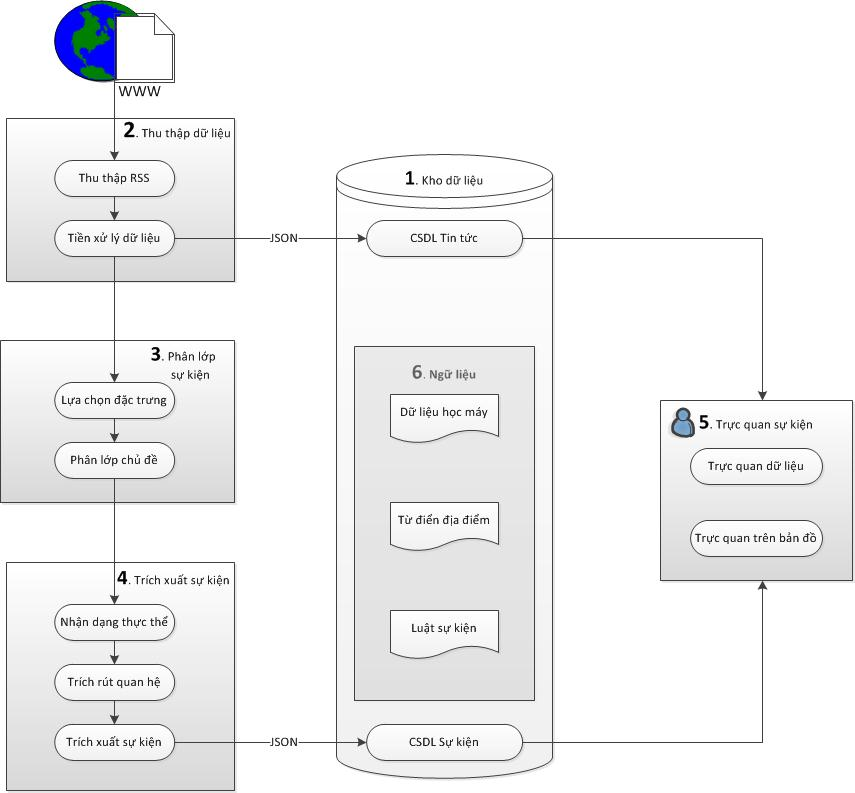
\includegraphics[ width=0.65\textwidth]{img/hugosystem}
		%\caption{Re--tweet}
		\label{fig:model}
	\end{figure}
\end{frame}
  \againframe<2->[plain]{zooms}

  \subsection{Demo hệ thống}
  \begin{frame}
      \begin{figure}[ht]
		\centering
		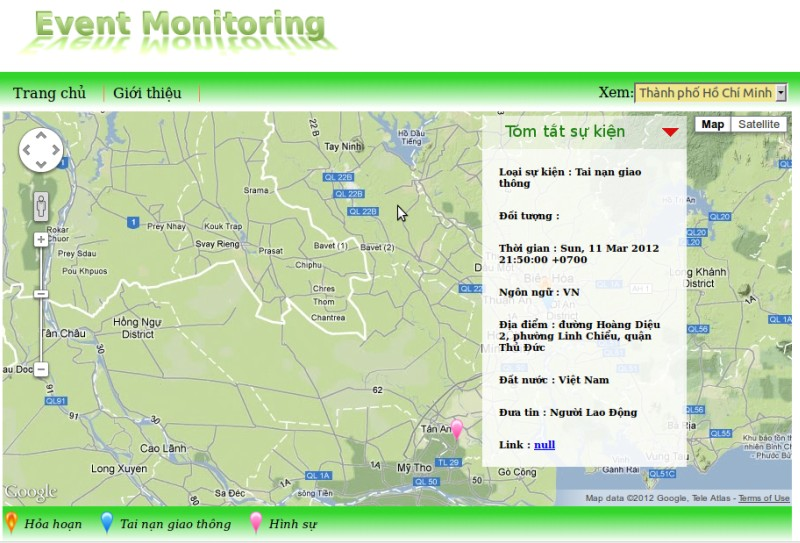
\includegraphics[width=4in, height=2.5in]{img/map1}
		%\caption{Re--tweet}
		\label{fig:model}
	\end{figure}

      \end{frame}












%\begin{frame}
%\frametitle{Re--tweet}
%\begin{columns}
%\column{2.0in}
%\begin{itemize}
%\item B nhìn thấy tweet của A và chuyển tiếp tweet đó những người "follow" B bằng cách re--tweet
%\medskip
%\item Xem xét quá trình re--tweet sẽ thiết lập được luồng thông tin
%\end{itemize}
%\column{2.0in}

%\begin{figure}[ht]
%\centering
%\includegraphics[height=1.8in,width=1.5in]{img/re}
%\caption{Re--tweet}
%\label{fig:url}
%\end{figure}

%\end{columns}

%\end{frame}

%Summary
\section*{}

\begin{frame}{Tổng kết}
\begin{itemize}
\item Các khái niệm cơ bản về mạng xã hội, phương tiện xã hội
\medskip
\item Đặc tính cơ bản của mạng xã hội
\medskip
\item Giám sát luồng thông tin trong mạng xã hội
\medskip
\item Ví dụ giám sát luồng thông tin qua phương tiện xã hội Twitter
\end{itemize}
\end{frame}

\begin{frame}
\begin{center}
\Huge{\duong{\textsc{CÂU HỎI???}}}
\end{center}
\end{frame}

\begin{frame}
\begin{center}
\Huge{\duong{\textsc{Cảm ơn thầy và các bạn đã quan tâm theo dõi!}}}
\end{center}
\end{frame}



\end{document}
